\documentclass[twoside]{book}

% Packages required by doxygen
\usepackage{fixltx2e}
\usepackage{calc}
\usepackage{doxygen}
\usepackage[export]{adjustbox} % also loads graphicx
\usepackage{graphicx}
\usepackage[utf8]{inputenc}
\usepackage{makeidx}
\usepackage{multicol}
\usepackage{multirow}
\PassOptionsToPackage{warn}{textcomp}
\usepackage{textcomp}
\usepackage[nointegrals]{wasysym}
\usepackage[table]{xcolor}

% Font selection
\usepackage[T1]{fontenc}
\usepackage[scaled=.90]{helvet}
\usepackage{courier}
\usepackage{amssymb}
\usepackage{sectsty}
\renewcommand{\familydefault}{\sfdefault}
\allsectionsfont{%
  \fontseries{bc}\selectfont%
  \color{darkgray}%
}
\renewcommand{\DoxyLabelFont}{%
  \fontseries{bc}\selectfont%
  \color{darkgray}%
}
\newcommand{\+}{\discretionary{\mbox{\scriptsize$\hookleftarrow$}}{}{}}

% Page & text layout
\usepackage{geometry}
\geometry{%
  a4paper,%
  top=2.5cm,%
  bottom=2.5cm,%
  left=2.5cm,%
  right=2.5cm%
}
\tolerance=750
\hfuzz=15pt
\hbadness=750
\setlength{\emergencystretch}{15pt}
\setlength{\parindent}{0cm}
\setlength{\parskip}{3ex plus 2ex minus 2ex}
\makeatletter
\renewcommand{\paragraph}{%
  \@startsection{paragraph}{4}{0ex}{-1.0ex}{1.0ex}{%
    \normalfont\normalsize\bfseries\SS@parafont%
  }%
}
\renewcommand{\subparagraph}{%
  \@startsection{subparagraph}{5}{0ex}{-1.0ex}{1.0ex}{%
    \normalfont\normalsize\bfseries\SS@subparafont%
  }%
}
\makeatother

% Headers & footers
\usepackage{fancyhdr}
\pagestyle{fancyplain}
\fancyhead[LE]{\fancyplain{}{\bfseries\thepage}}
\fancyhead[CE]{\fancyplain{}{}}
\fancyhead[RE]{\fancyplain{}{\bfseries\leftmark}}
\fancyhead[LO]{\fancyplain{}{\bfseries\rightmark}}
\fancyhead[CO]{\fancyplain{}{}}
\fancyhead[RO]{\fancyplain{}{\bfseries\thepage}}
\fancyfoot[LE]{\fancyplain{}{}}
\fancyfoot[CE]{\fancyplain{}{}}
\fancyfoot[RE]{\fancyplain{}{\bfseries\scriptsize Generated by Doxygen }}
\fancyfoot[LO]{\fancyplain{}{\bfseries\scriptsize Generated by Doxygen }}
\fancyfoot[CO]{\fancyplain{}{}}
\fancyfoot[RO]{\fancyplain{}{}}
\renewcommand{\footrulewidth}{0.4pt}
\renewcommand{\chaptermark}[1]{%
  \markboth{#1}{}%
}
\renewcommand{\sectionmark}[1]{%
  \markright{\thesection\ #1}%
}

% Indices & bibliography
\usepackage{natbib}
\usepackage[titles]{tocloft}
\setcounter{tocdepth}{3}
\setcounter{secnumdepth}{5}
\makeindex

% Hyperlinks (required, but should be loaded last)
\usepackage{ifpdf}
\ifpdf
  \usepackage[pdftex,pagebackref=true]{hyperref}
\else
  \usepackage[ps2pdf,pagebackref=true]{hyperref}
\fi
\hypersetup{%
  colorlinks=true,%
  linkcolor=blue,%
  citecolor=blue,%
  unicode%
}

% Custom commands
\newcommand{\clearemptydoublepage}{%
  \newpage{\pagestyle{empty}\cleardoublepage}%
}

\usepackage{caption}
\captionsetup{labelsep=space,justification=centering,font={bf},singlelinecheck=off,skip=4pt,position=top}

%===== C O N T E N T S =====

\begin{document}

% Titlepage & ToC
\hypersetup{pageanchor=false,
             bookmarksnumbered=true,
             pdfencoding=unicode
            }
\pagenumbering{roman}
\begin{titlepage}
\vspace*{7cm}
\begin{center}%
{\Large Heisprosjekt -\/ Gruppe 22 }\\
\vspace*{1cm}
{\large Generated by Doxygen 1.8.11}\\
\end{center}
\end{titlepage}
\clearemptydoublepage
\tableofcontents
\clearemptydoublepage
\pagenumbering{arabic}
\hypersetup{pageanchor=true}

%--- Begin generated contents ---
\chapter{Data Structure Index}
\section{Data Structures}
Here are the data structures with brief descriptions\+:\begin{DoxyCompactList}
\item\contentsline{section}{\hyperlink{structstatus__stat}{status\+\_\+stat} \\*Keeps track of the elevator status }{\pageref{structstatus__stat}}{}
\end{DoxyCompactList}

\chapter{File Index}
\section{File List}
Here is a list of all documented files with brief descriptions\+:\begin{DoxyCompactList}
\item\contentsline{section}{source/{\bfseries button\+\_\+operations.\+c} }{\pageref{button__operations_8c}}{}
\item\contentsline{section}{source/\hyperlink{button__operations_8h}{button\+\_\+operations.\+h} \\*Includes funtions for setting and resetting the button lamps on the elevator panel }{\pageref{button__operations_8h}}{}
\item\contentsline{section}{source/{\bfseries channels.\+h} }{\pageref{channels_8h}}{}
\item\contentsline{section}{source/{\bfseries controller.\+c} }{\pageref{controller_8c}}{}
\item\contentsline{section}{source/\hyperlink{controller_8h}{controller.\+h} \\*The controller file constists of two global structs for keeping track of the elevator status and the state of the elevator. Funtions for reseting, stopping, running, executing and initializing the elevator as well as functions for updtating the status and state are also included. The main logic of the elvator lies within the \hyperlink{controller_8h_a29eb4c73c46dfbbbe1c9f908b781192c}{run\+\_\+elevator()} function }{\pageref{controller_8h}}{}
\item\contentsline{section}{source/{\bfseries door.\+c} }{\pageref{door_8c}}{}
\item\contentsline{section}{source/\hyperlink{door_8h}{door.\+h} \\*The door file includes functions for opening and closing the door. There is also implemented a three second time delay for holding the door open }{\pageref{door_8h}}{}
\item\contentsline{section}{source/{\bfseries elev.\+c} }{\pageref{elev_8c}}{}
\item\contentsline{section}{source/{\bfseries elev.\+h} }{\pageref{elev_8h}}{}
\item\contentsline{section}{source/{\bfseries io.\+c} }{\pageref{io_8c}}{}
\item\contentsline{section}{source/{\bfseries io.\+h} }{\pageref{io_8h}}{}
\item\contentsline{section}{source/{\bfseries main.\+c} }{\pageref{main_8c}}{}
\item\contentsline{section}{source/{\bfseries queue.\+c} }{\pageref{queue_8c}}{}
\item\contentsline{section}{source/\hyperlink{queue_8h}{queue.\+h} \\*The queue file includes funtions used to manipulate the queue for the elevator, determine direction based on elements in queue and check if the queue is empty }{\pageref{queue_8h}}{}
\end{DoxyCompactList}

\chapter{Data Structure Documentation}
\hypertarget{structstatus__stat}{}\section{status\+\_\+stat Struct Reference}
\label{structstatus__stat}\index{status\+\_\+stat@{status\+\_\+stat}}


Keeps track of the elevator status.  




{\ttfamily \#include $<$controller.\+h$>$}

\subsection*{Data Fields}
\begin{DoxyCompactItemize}
\item 
int \hyperlink{structstatus__stat_ad8dbbabdd11cad499360434a98fc4800}{queue} \mbox{[}4\mbox{]}\mbox{[}3\mbox{]}
\item 
elev\+\_\+motor\+\_\+direction\+\_\+t \hyperlink{structstatus__stat_a86473b5ad6efc13580fd36cd74490f8f}{dir}
\item 
elev\+\_\+motor\+\_\+direction\+\_\+t \hyperlink{structstatus__stat_a57dbf007f4cf7b8d0b2872a99f5e6f62}{prev\+\_\+dir}
\item 
elev\+\_\+motor\+\_\+direction\+\_\+t \hyperlink{structstatus__stat_a9edb07751cab0af2679e323190e49762}{dir\+\_\+before\+\_\+stop}
\item 
int \hyperlink{structstatus__stat_afb8f4c42e97ba9ede62ba17a2f157757}{current\+\_\+floor}
\item 
int \hyperlink{structstatus__stat_a4ccf00bc4cb3475a93c3bf5eb2a9a819}{prev\+\_\+floor}
\item 
\hyperlink{controller_8h_ada5afb1226f3d604e014674fa0448069}{states} \hyperlink{structstatus__stat_ac485f83fea98239454b3ec1eb49e29cc}{state}
\end{DoxyCompactItemize}


\subsection{Detailed Description}
Keeps track of the elevator status. 

Definition at line 28 of file controller.\+h.



\subsection{Field Documentation}
\index{status\+\_\+stat@{status\+\_\+stat}!current\+\_\+floor@{current\+\_\+floor}}
\index{current\+\_\+floor@{current\+\_\+floor}!status\+\_\+stat@{status\+\_\+stat}}
\subsubsection[{\texorpdfstring{current\+\_\+floor}{current_floor}}]{\setlength{\rightskip}{0pt plus 5cm}int status\+\_\+stat\+::current\+\_\+floor}\hypertarget{structstatus__stat_afb8f4c42e97ba9ede62ba17a2f157757}{}\label{structstatus__stat_afb8f4c42e97ba9ede62ba17a2f157757}
Stores the current floor, and is -\/1 when the elevator is between floors 

Definition at line 33 of file controller.\+h.

\index{status\+\_\+stat@{status\+\_\+stat}!dir@{dir}}
\index{dir@{dir}!status\+\_\+stat@{status\+\_\+stat}}
\subsubsection[{\texorpdfstring{dir}{dir}}]{\setlength{\rightskip}{0pt plus 5cm}elev\+\_\+motor\+\_\+direction\+\_\+t status\+\_\+stat\+::dir}\hypertarget{structstatus__stat_a86473b5ad6efc13580fd36cd74490f8f}{}\label{structstatus__stat_a86473b5ad6efc13580fd36cd74490f8f}
The current direction which is uptated regularly 

Definition at line 30 of file controller.\+h.

\index{status\+\_\+stat@{status\+\_\+stat}!dir\+\_\+before\+\_\+stop@{dir\+\_\+before\+\_\+stop}}
\index{dir\+\_\+before\+\_\+stop@{dir\+\_\+before\+\_\+stop}!status\+\_\+stat@{status\+\_\+stat}}
\subsubsection[{\texorpdfstring{dir\+\_\+before\+\_\+stop}{dir_before_stop}}]{\setlength{\rightskip}{0pt plus 5cm}elev\+\_\+motor\+\_\+direction\+\_\+t status\+\_\+stat\+::dir\+\_\+before\+\_\+stop}\hypertarget{structstatus__stat_a9edb07751cab0af2679e323190e49762}{}\label{structstatus__stat_a9edb07751cab0af2679e323190e49762}
Used to determine direction when elevator stop button is pressed several times between floors 

Definition at line 32 of file controller.\+h.

\index{status\+\_\+stat@{status\+\_\+stat}!prev\+\_\+dir@{prev\+\_\+dir}}
\index{prev\+\_\+dir@{prev\+\_\+dir}!status\+\_\+stat@{status\+\_\+stat}}
\subsubsection[{\texorpdfstring{prev\+\_\+dir}{prev_dir}}]{\setlength{\rightskip}{0pt plus 5cm}elev\+\_\+motor\+\_\+direction\+\_\+t status\+\_\+stat\+::prev\+\_\+dir}\hypertarget{structstatus__stat_a57dbf007f4cf7b8d0b2872a99f5e6f62}{}\label{structstatus__stat_a57dbf007f4cf7b8d0b2872a99f5e6f62}
Stores the previous direction different from the current direction 

Definition at line 31 of file controller.\+h.

\index{status\+\_\+stat@{status\+\_\+stat}!prev\+\_\+floor@{prev\+\_\+floor}}
\index{prev\+\_\+floor@{prev\+\_\+floor}!status\+\_\+stat@{status\+\_\+stat}}
\subsubsection[{\texorpdfstring{prev\+\_\+floor}{prev_floor}}]{\setlength{\rightskip}{0pt plus 5cm}int status\+\_\+stat\+::prev\+\_\+floor}\hypertarget{structstatus__stat_a4ccf00bc4cb3475a93c3bf5eb2a9a819}{}\label{structstatus__stat_a4ccf00bc4cb3475a93c3bf5eb2a9a819}
Stores current floor. Only updated when the elevatro passes or stops on a floor 

Definition at line 34 of file controller.\+h.

\index{status\+\_\+stat@{status\+\_\+stat}!queue@{queue}}
\index{queue@{queue}!status\+\_\+stat@{status\+\_\+stat}}
\subsubsection[{\texorpdfstring{queue}{queue}}]{\setlength{\rightskip}{0pt plus 5cm}int status\+\_\+stat\+::queue\mbox{[}4\mbox{]}\mbox{[}3\mbox{]}}\hypertarget{structstatus__stat_ad8dbbabdd11cad499360434a98fc4800}{}\label{structstatus__stat_ad8dbbabdd11cad499360434a98fc4800}
A 4x3 matrix which to keep track of floor orders from the different types of buttons 

Definition at line 29 of file controller.\+h.

\index{status\+\_\+stat@{status\+\_\+stat}!state@{state}}
\index{state@{state}!status\+\_\+stat@{status\+\_\+stat}}
\subsubsection[{\texorpdfstring{state}{state}}]{\setlength{\rightskip}{0pt plus 5cm}{\bf states} status\+\_\+stat\+::state}\hypertarget{structstatus__stat_ac485f83fea98239454b3ec1eb49e29cc}{}\label{structstatus__stat_ac485f83fea98239454b3ec1eb49e29cc}
Keeps track on the state the elevator is in 

Definition at line 35 of file controller.\+h.



The documentation for this struct was generated from the following file\+:\begin{DoxyCompactItemize}
\item 
source/\hyperlink{controller_8h}{controller.\+h}\end{DoxyCompactItemize}

\chapter{File Documentation}
\hypertarget{button__operations_8h}{}\section{source/button\+\_\+operations.h File Reference}
\label{button__operations_8h}\index{source/button\+\_\+operations.\+h@{source/button\+\_\+operations.\+h}}


Includes funtions for setting and resetting the button lamps on the elevator panel.  


This graph shows which files directly or indirectly include this file\+:
\nopagebreak
\begin{figure}[H]
\begin{center}
\leavevmode
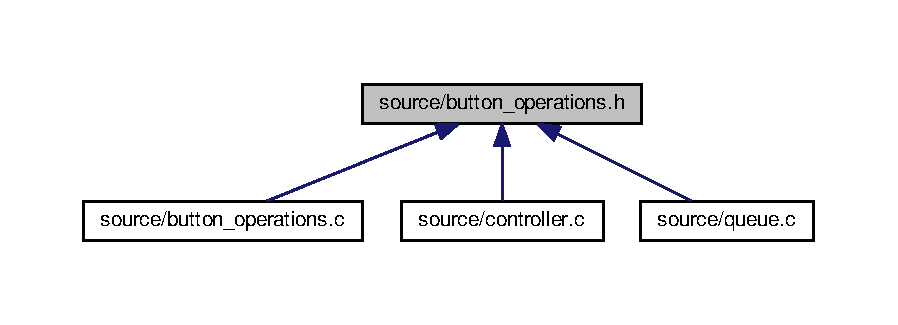
\includegraphics[width=350pt]{button__operations_8h__dep__incl}
\end{center}
\end{figure}
\subsection*{Functions}
\begin{DoxyCompactItemize}
\item 
void \hyperlink{button__operations_8h_aadc3230a57792e94e182ab8b62817aef}{read\+\_\+set\+\_\+button\+\_\+lights} ()\hypertarget{button__operations_8h_aadc3230a57792e94e182ab8b62817aef}{}\label{button__operations_8h_aadc3230a57792e94e182ab8b62817aef}

\begin{DoxyCompactList}\small\item\em Reads the button the button signals by going through the queue and sets the light if the value in the array is 1. \end{DoxyCompactList}\item 
void \hyperlink{button__operations_8h_a9f5b137f9f0180345dae1d38495a2f03}{reset\+\_\+all\+\_\+lights\+\_\+but\+\_\+stop} ()\hypertarget{button__operations_8h_a9f5b137f9f0180345dae1d38495a2f03}{}\label{button__operations_8h_a9f5b137f9f0180345dae1d38495a2f03}

\begin{DoxyCompactList}\small\item\em Goes through the queue and resets all of the button lights Only the stop button light is still set. \end{DoxyCompactList}\item 
void \hyperlink{button__operations_8h_a1130869137c48307c82c10d323b17a78}{reset\+\_\+current\+\_\+floor\+\_\+light} (int flr)
\begin{DoxyCompactList}\small\item\em Goes through the queue and resets all of the button lights on the floor which is taken in as an argument in the function. \end{DoxyCompactList}\end{DoxyCompactItemize}


\subsection{Detailed Description}
Includes funtions for setting and resetting the button lamps on the elevator panel. 



\subsection{Function Documentation}
\index{button\+\_\+operations.\+h@{button\+\_\+operations.\+h}!reset\+\_\+current\+\_\+floor\+\_\+light@{reset\+\_\+current\+\_\+floor\+\_\+light}}
\index{reset\+\_\+current\+\_\+floor\+\_\+light@{reset\+\_\+current\+\_\+floor\+\_\+light}!button\+\_\+operations.\+h@{button\+\_\+operations.\+h}}
\subsubsection[{\texorpdfstring{reset\+\_\+current\+\_\+floor\+\_\+light(int flr)}{reset_current_floor_light(int flr)}}]{\setlength{\rightskip}{0pt plus 5cm}void reset\+\_\+current\+\_\+floor\+\_\+light (
\begin{DoxyParamCaption}
\item[{int}]{flr}
\end{DoxyParamCaption}
)}\hypertarget{button__operations_8h_a1130869137c48307c82c10d323b17a78}{}\label{button__operations_8h_a1130869137c48307c82c10d323b17a78}


Goes through the queue and resets all of the button lights on the floor which is taken in as an argument in the function. 


\begin{DoxyParams}[1]{Parameters}
\mbox{\tt in}  & {\em flr} & -\/ The value of the relevant floor. \\
\hline
\end{DoxyParams}


Definition at line 28 of file button\+\_\+operations.\+c.


\hypertarget{controller_8h}{}\section{source/controller.h File Reference}
\label{controller_8h}\index{source/controller.\+h@{source/controller.\+h}}


The controller file constists of two global structs for keeping track of the elevator status and the state of the elevator. Funtions for reseting, stopping, running, executing and initializing the elevator as well as functions for updtating the status and state are also included. The main logic of the elvator lies within the \hyperlink{controller_8h_a29eb4c73c46dfbbbe1c9f908b781192c}{run\+\_\+elevator()} function.  


{\ttfamily \#include \char`\"{}elev.\+h\char`\"{}}\\*
Include dependency graph for controller.\+h\+:
\nopagebreak
\begin{figure}[H]
\begin{center}
\leavevmode
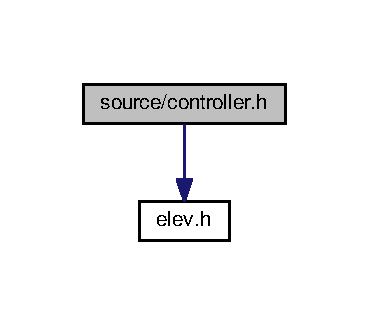
\includegraphics[width=177pt]{controller_8h__incl}
\end{center}
\end{figure}
This graph shows which files directly or indirectly include this file\+:
\nopagebreak
\begin{figure}[H]
\begin{center}
\leavevmode
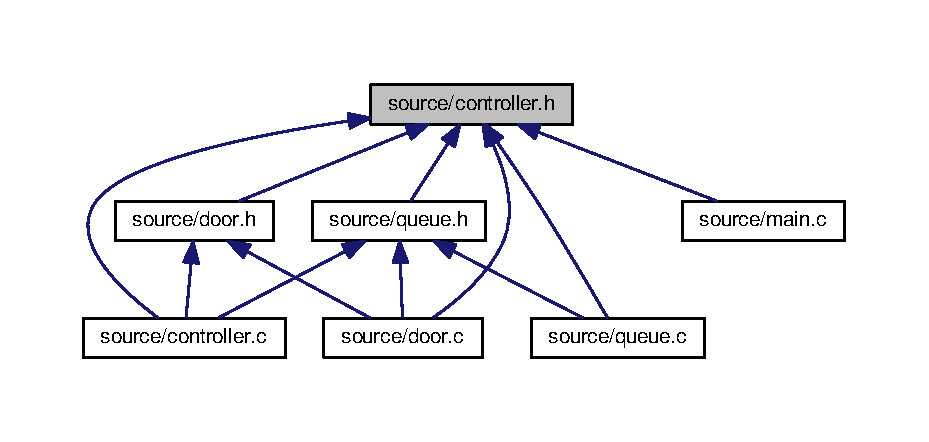
\includegraphics[width=350pt]{controller_8h__dep__incl}
\end{center}
\end{figure}
\subsection*{Data Structures}
\begin{DoxyCompactItemize}
\item 
struct \hyperlink{structstatus__stat}{status\+\_\+stat}
\begin{DoxyCompactList}\small\item\em Keeps track of the elevator status. \end{DoxyCompactList}\end{DoxyCompactItemize}
\subsection*{Typedefs}
\begin{DoxyCompactItemize}
\item 
typedef enum \hyperlink{controller_8h_a798d1d3831b58bf27f3c5853317502b5}{states\+\_\+stat} \hyperlink{controller_8h_ada5afb1226f3d604e014674fa0448069}{states}\hypertarget{controller_8h_ada5afb1226f3d604e014674fa0448069}{}\label{controller_8h_ada5afb1226f3d604e014674fa0448069}

\begin{DoxyCompactList}\small\item\em Holds all the states included within the state-\/ machine. \end{DoxyCompactList}\item 
typedef struct \hyperlink{structstatus__stat}{status\+\_\+stat} \hyperlink{controller_8h_a7f15c77206bc6cf59d763bb72cc381e6}{status}\hypertarget{controller_8h_a7f15c77206bc6cf59d763bb72cc381e6}{}\label{controller_8h_a7f15c77206bc6cf59d763bb72cc381e6}

\begin{DoxyCompactList}\small\item\em Keeps track of the elevator status. \end{DoxyCompactList}\end{DoxyCompactItemize}
\subsection*{Enumerations}
\begin{DoxyCompactItemize}
\item 
enum \hyperlink{controller_8h_a798d1d3831b58bf27f3c5853317502b5}{states\+\_\+stat} \{ \hyperlink{controller_8h_a798d1d3831b58bf27f3c5853317502b5ae4634ae4352b512b38c5da9dc1610ca6}{S\+T\+A\+N\+D\+BY}, 
\hyperlink{controller_8h_a798d1d3831b58bf27f3c5853317502b5a79a322ccb4b29b85b3cab52dbccefd17}{W\+A\+IT}, 
\hyperlink{controller_8h_a798d1d3831b58bf27f3c5853317502b5a679ee5320d66c8322e310daeb2ee99b8}{S\+T\+OP}, 
\hyperlink{controller_8h_a798d1d3831b58bf27f3c5853317502b5ae1bb1460cb779888412e634e983be161}{A\+C\+T\+I\+ON}
 \}\begin{DoxyCompactList}\small\item\em Holds all the states included within the state-\/ machine. \end{DoxyCompactList}
\end{DoxyCompactItemize}
\subsection*{Functions}
\begin{DoxyCompactItemize}
\item 
void \hyperlink{controller_8h_a242b33d09d6a2e733a219bb9342bddcb}{reset\+\_\+elevator} (\hyperlink{controller_8h_a7f15c77206bc6cf59d763bb72cc381e6}{status} $\ast$elevator)
\begin{DoxyCompactList}\small\item\em Resets all elements in queue, and resets all enabled lamps. Updates prev\+\_\+dir within status struct. \end{DoxyCompactList}\item 
void \hyperlink{controller_8h_a2a9af841252d044dd8da2f48ca32e776}{stop\+\_\+elevator} (\hyperlink{controller_8h_a7f15c77206bc6cf59d763bb72cc381e6}{status} $\ast$elevator)
\begin{DoxyCompactList}\small\item\em Sets and updates status of motor direction to D\+I\+R\+N\+\_\+\+S\+T\+OP, resets the elevator and opens the door for three seconds if the elevator is not between floors. \end{DoxyCompactList}\item 
void \hyperlink{controller_8h_a29eb4c73c46dfbbbe1c9f908b781192c}{run\+\_\+elevator} (\hyperlink{controller_8h_a7f15c77206bc6cf59d763bb72cc381e6}{status} $\ast$elevator)
\begin{DoxyCompactList}\small\item\em Contains the complete state machine of the elevator. \end{DoxyCompactList}\item 
void \hyperlink{controller_8h_adcab175bee116f39d33681fd94d6b9bf}{read\+\_\+set\+\_\+motor\+\_\+dir} (\hyperlink{controller_8h_a7f15c77206bc6cf59d763bb72cc381e6}{status} $\ast$elevator)
\begin{DoxyCompactList}\small\item\em Determines a new direction based on the elevator orders and the elevator status. \end{DoxyCompactList}\item 
void \hyperlink{controller_8h_a5b96c2d6030e1c72f70ccf84f633b344}{initialize\+\_\+elevator} (\hyperlink{controller_8h_a7f15c77206bc6cf59d763bb72cc381e6}{status} $\ast$elevator)
\begin{DoxyCompactList}\small\item\em Initializes the the start state and status of the elvator. Forces the elevator to the first floor, and keeps the door closed. \end{DoxyCompactList}\item 
void \hyperlink{controller_8h_a406460bef998b9f9452622bda738926c}{set\+\_\+current\+\_\+floor} (\hyperlink{controller_8h_a7f15c77206bc6cf59d763bb72cc381e6}{status} $\ast$elevator)
\begin{DoxyCompactList}\small\item\em Sets current floor in the status struct based on floor sensor activity. \end{DoxyCompactList}\item 
void \hyperlink{controller_8h_a1cbe8b7e0ea6e4dd45868d7964f11bef}{stop\+\_\+on\+\_\+floor\+\_\+if\+\_\+ordered} (\hyperlink{controller_8h_a7f15c77206bc6cf59d763bb72cc381e6}{status} $\ast$elevator)
\begin{DoxyCompactList}\small\item\em Makes the elevator stop, when it passes a floor with an avtive order. Updates status and state. \end{DoxyCompactList}\item 
void \hyperlink{controller_8h_a1d2c99e9972a3266a724203c1403b638}{reset\+\_\+floor} (\hyperlink{controller_8h_a7f15c77206bc6cf59d763bb72cc381e6}{status} $\ast$elevator)
\begin{DoxyCompactList}\small\item\em Resets lamps and orders assosiated with the floor where the elevator stops. \end{DoxyCompactList}\end{DoxyCompactItemize}


\subsection{Detailed Description}
The controller file constists of two global structs for keeping track of the elevator status and the state of the elevator. Funtions for reseting, stopping, running, executing and initializing the elevator as well as functions for updtating the status and state are also included. The main logic of the elvator lies within the \hyperlink{controller_8h_a29eb4c73c46dfbbbe1c9f908b781192c}{run\+\_\+elevator()} function. 



\subsection{Enumeration Type Documentation}
\index{controller.\+h@{controller.\+h}!states\+\_\+stat@{states\+\_\+stat}}
\index{states\+\_\+stat@{states\+\_\+stat}!controller.\+h@{controller.\+h}}
\subsubsection[{\texorpdfstring{states\+\_\+stat}{states_stat}}]{\setlength{\rightskip}{0pt plus 5cm}enum {\bf states\+\_\+stat}}\hypertarget{controller_8h_a798d1d3831b58bf27f3c5853317502b5}{}\label{controller_8h_a798d1d3831b58bf27f3c5853317502b5}


Holds all the states included within the state-\/ machine. 

\begin{Desc}
\item[Enumerator]\par
\begin{description}
\index{S\+T\+A\+N\+D\+BY@{S\+T\+A\+N\+D\+BY}!controller.\+h@{controller.\+h}}\index{controller.\+h@{controller.\+h}!S\+T\+A\+N\+D\+BY@{S\+T\+A\+N\+D\+BY}}\item[{\em 
S\+T\+A\+N\+D\+BY\hypertarget{controller_8h_a798d1d3831b58bf27f3c5853317502b5ae4634ae4352b512b38c5da9dc1610ca6}{}\label{controller_8h_a798d1d3831b58bf27f3c5853317502b5ae4634ae4352b512b38c5da9dc1610ca6}
}]The state where the motor direction is determined \index{W\+A\+IT@{W\+A\+IT}!controller.\+h@{controller.\+h}}\index{controller.\+h@{controller.\+h}!W\+A\+IT@{W\+A\+IT}}\item[{\em 
W\+A\+IT\hypertarget{controller_8h_a798d1d3831b58bf27f3c5853317502b5a79a322ccb4b29b85b3cab52dbccefd17}{}\label{controller_8h_a798d1d3831b58bf27f3c5853317502b5a79a322ccb4b29b85b3cab52dbccefd17}
}]Here the door stays open for three seconds \index{S\+T\+OP@{S\+T\+OP}!controller.\+h@{controller.\+h}}\index{controller.\+h@{controller.\+h}!S\+T\+OP@{S\+T\+OP}}\item[{\em 
S\+T\+OP\hypertarget{controller_8h_a798d1d3831b58bf27f3c5853317502b5a679ee5320d66c8322e310daeb2ee99b8}{}\label{controller_8h_a798d1d3831b58bf27f3c5853317502b5a679ee5320d66c8322e310daeb2ee99b8}
}]Sets the state to S\+T\+A\+N\+D\+BY \index{A\+C\+T\+I\+ON@{A\+C\+T\+I\+ON}!controller.\+h@{controller.\+h}}\index{controller.\+h@{controller.\+h}!A\+C\+T\+I\+ON@{A\+C\+T\+I\+ON}}\item[{\em 
A\+C\+T\+I\+ON\hypertarget{controller_8h_a798d1d3831b58bf27f3c5853317502b5ae1bb1460cb779888412e634e983be161}{}\label{controller_8h_a798d1d3831b58bf27f3c5853317502b5ae1bb1460cb779888412e634e983be161}
}]Looks for orders and act upon it. Upates queue and status \end{description}
\end{Desc}


Definition at line 17 of file controller.\+h.



\subsection{Function Documentation}
\index{controller.\+h@{controller.\+h}!initialize\+\_\+elevator@{initialize\+\_\+elevator}}
\index{initialize\+\_\+elevator@{initialize\+\_\+elevator}!controller.\+h@{controller.\+h}}
\subsubsection[{\texorpdfstring{initialize\+\_\+elevator(status $\ast$elevator)}{initialize_elevator(status *elevator)}}]{\setlength{\rightskip}{0pt plus 5cm}void initialize\+\_\+elevator (
\begin{DoxyParamCaption}
\item[{{\bf status} $\ast$}]{elevator}
\end{DoxyParamCaption}
)}\hypertarget{controller_8h_a5b96c2d6030e1c72f70ccf84f633b344}{}\label{controller_8h_a5b96c2d6030e1c72f70ccf84f633b344}


Initializes the the start state and status of the elvator. Forces the elevator to the first floor, and keeps the door closed. 


\begin{DoxyParams}[1]{Parameters}
\mbox{\tt in,out}  & {\em status$\ast$} & elevator Struct for elevator status. \\
\hline
\end{DoxyParams}


Definition at line 126 of file controller.\+c.

\index{controller.\+h@{controller.\+h}!read\+\_\+set\+\_\+motor\+\_\+dir@{read\+\_\+set\+\_\+motor\+\_\+dir}}
\index{read\+\_\+set\+\_\+motor\+\_\+dir@{read\+\_\+set\+\_\+motor\+\_\+dir}!controller.\+h@{controller.\+h}}
\subsubsection[{\texorpdfstring{read\+\_\+set\+\_\+motor\+\_\+dir(status $\ast$elevator)}{read_set_motor_dir(status *elevator)}}]{\setlength{\rightskip}{0pt plus 5cm}void read\+\_\+set\+\_\+motor\+\_\+dir (
\begin{DoxyParamCaption}
\item[{{\bf status} $\ast$}]{elevator}
\end{DoxyParamCaption}
)}\hypertarget{controller_8h_adcab175bee116f39d33681fd94d6b9bf}{}\label{controller_8h_adcab175bee116f39d33681fd94d6b9bf}


Determines a new direction based on the elevator orders and the elevator status. 


\begin{DoxyParams}[1]{Parameters}
\mbox{\tt in,out}  & {\em status$\ast$} & elevator Struct for elevator status. \\
\hline
\end{DoxyParams}


Definition at line 39 of file controller.\+c.

\index{controller.\+h@{controller.\+h}!reset\+\_\+elevator@{reset\+\_\+elevator}}
\index{reset\+\_\+elevator@{reset\+\_\+elevator}!controller.\+h@{controller.\+h}}
\subsubsection[{\texorpdfstring{reset\+\_\+elevator(status $\ast$elevator)}{reset_elevator(status *elevator)}}]{\setlength{\rightskip}{0pt plus 5cm}void reset\+\_\+elevator (
\begin{DoxyParamCaption}
\item[{{\bf status} $\ast$}]{elevator}
\end{DoxyParamCaption}
)}\hypertarget{controller_8h_a242b33d09d6a2e733a219bb9342bddcb}{}\label{controller_8h_a242b33d09d6a2e733a219bb9342bddcb}


Resets all elements in queue, and resets all enabled lamps. Updates prev\+\_\+dir within status struct. 


\begin{DoxyParams}[1]{Parameters}
\mbox{\tt in,out}  & {\em status$\ast$} & elevator Struct for elevator status. \\
\hline
\end{DoxyParams}


Definition at line 11 of file controller.\+c.

\index{controller.\+h@{controller.\+h}!reset\+\_\+floor@{reset\+\_\+floor}}
\index{reset\+\_\+floor@{reset\+\_\+floor}!controller.\+h@{controller.\+h}}
\subsubsection[{\texorpdfstring{reset\+\_\+floor(status $\ast$elevator)}{reset_floor(status *elevator)}}]{\setlength{\rightskip}{0pt plus 5cm}void reset\+\_\+floor (
\begin{DoxyParamCaption}
\item[{{\bf status} $\ast$}]{elevator}
\end{DoxyParamCaption}
)}\hypertarget{controller_8h_a1d2c99e9972a3266a724203c1403b638}{}\label{controller_8h_a1d2c99e9972a3266a724203c1403b638}


Resets lamps and orders assosiated with the floor where the elevator stops. 


\begin{DoxyParams}[1]{Parameters}
\mbox{\tt in,out}  & {\em status$\ast$} & elevator Struct for elevator status. \\
\hline
\end{DoxyParams}


Definition at line 75 of file controller.\+c.

\index{controller.\+h@{controller.\+h}!run\+\_\+elevator@{run\+\_\+elevator}}
\index{run\+\_\+elevator@{run\+\_\+elevator}!controller.\+h@{controller.\+h}}
\subsubsection[{\texorpdfstring{run\+\_\+elevator(status $\ast$elevator)}{run_elevator(status *elevator)}}]{\setlength{\rightskip}{0pt plus 5cm}void run\+\_\+elevator (
\begin{DoxyParamCaption}
\item[{{\bf status} $\ast$}]{elevator}
\end{DoxyParamCaption}
)}\hypertarget{controller_8h_a29eb4c73c46dfbbbe1c9f908b781192c}{}\label{controller_8h_a29eb4c73c46dfbbbe1c9f908b781192c}


Contains the complete state machine of the elevator. 


\begin{DoxyParams}[1]{Parameters}
\mbox{\tt in,out}  & {\em status$\ast$} & elevator Struct for elevator status. \\
\hline
\end{DoxyParams}


Definition at line 88 of file controller.\+c.

\index{controller.\+h@{controller.\+h}!set\+\_\+current\+\_\+floor@{set\+\_\+current\+\_\+floor}}
\index{set\+\_\+current\+\_\+floor@{set\+\_\+current\+\_\+floor}!controller.\+h@{controller.\+h}}
\subsubsection[{\texorpdfstring{set\+\_\+current\+\_\+floor(status $\ast$elevator)}{set_current_floor(status *elevator)}}]{\setlength{\rightskip}{0pt plus 5cm}void set\+\_\+current\+\_\+floor (
\begin{DoxyParamCaption}
\item[{{\bf status} $\ast$}]{elevator}
\end{DoxyParamCaption}
)}\hypertarget{controller_8h_a406460bef998b9f9452622bda738926c}{}\label{controller_8h_a406460bef998b9f9452622bda738926c}


Sets current floor in the status struct based on floor sensor activity. 


\begin{DoxyParams}[1]{Parameters}
\mbox{\tt in,out}  & {\em status$\ast$} & elevator Struct for elevator status. \\
\hline
\end{DoxyParams}


Definition at line 51 of file controller.\+c.

\index{controller.\+h@{controller.\+h}!stop\+\_\+elevator@{stop\+\_\+elevator}}
\index{stop\+\_\+elevator@{stop\+\_\+elevator}!controller.\+h@{controller.\+h}}
\subsubsection[{\texorpdfstring{stop\+\_\+elevator(status $\ast$elevator)}{stop_elevator(status *elevator)}}]{\setlength{\rightskip}{0pt plus 5cm}void stop\+\_\+elevator (
\begin{DoxyParamCaption}
\item[{{\bf status} $\ast$}]{elevator}
\end{DoxyParamCaption}
)}\hypertarget{controller_8h_a2a9af841252d044dd8da2f48ca32e776}{}\label{controller_8h_a2a9af841252d044dd8da2f48ca32e776}


Sets and updates status of motor direction to D\+I\+R\+N\+\_\+\+S\+T\+OP, resets the elevator and opens the door for three seconds if the elevator is not between floors. 


\begin{DoxyParams}[1]{Parameters}
\mbox{\tt in,out}  & {\em status$\ast$} & elevator Struct for elevator status. \\
\hline
\end{DoxyParams}


Definition at line 23 of file controller.\+c.

\index{controller.\+h@{controller.\+h}!stop\+\_\+on\+\_\+floor\+\_\+if\+\_\+ordered@{stop\+\_\+on\+\_\+floor\+\_\+if\+\_\+ordered}}
\index{stop\+\_\+on\+\_\+floor\+\_\+if\+\_\+ordered@{stop\+\_\+on\+\_\+floor\+\_\+if\+\_\+ordered}!controller.\+h@{controller.\+h}}
\subsubsection[{\texorpdfstring{stop\+\_\+on\+\_\+floor\+\_\+if\+\_\+ordered(status $\ast$elevator)}{stop_on_floor_if_ordered(status *elevator)}}]{\setlength{\rightskip}{0pt plus 5cm}void stop\+\_\+on\+\_\+floor\+\_\+if\+\_\+ordered (
\begin{DoxyParamCaption}
\item[{{\bf status} $\ast$}]{elevator}
\end{DoxyParamCaption}
)}\hypertarget{controller_8h_a1cbe8b7e0ea6e4dd45868d7964f11bef}{}\label{controller_8h_a1cbe8b7e0ea6e4dd45868d7964f11bef}


Makes the elevator stop, when it passes a floor with an avtive order. Updates status and state. 


\begin{DoxyParams}[1]{Parameters}
\mbox{\tt in,out}  & {\em status$\ast$} & elevator Struct for elevator status. \\
\hline
\end{DoxyParams}


Definition at line 59 of file controller.\+c.


\hypertarget{door_8h}{}\section{source/door.h File Reference}
\label{door_8h}\index{source/door.\+h@{source/door.\+h}}


The door file includes functions for opening and closing the door. There is also implemented a three second time delay for holding the door open.  


{\ttfamily \#include $<$stdbool.\+h$>$}\\*
{\ttfamily \#include \char`\"{}controller.\+h\char`\"{}}\\*
Include dependency graph for door.\+h\+:
\nopagebreak
\begin{figure}[H]
\begin{center}
\leavevmode
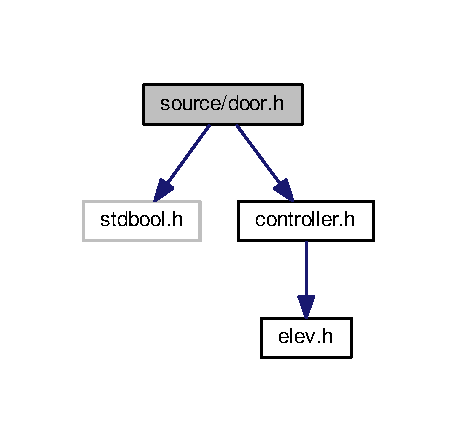
\includegraphics[width=220pt]{door_8h__incl}
\end{center}
\end{figure}
This graph shows which files directly or indirectly include this file\+:
\nopagebreak
\begin{figure}[H]
\begin{center}
\leavevmode
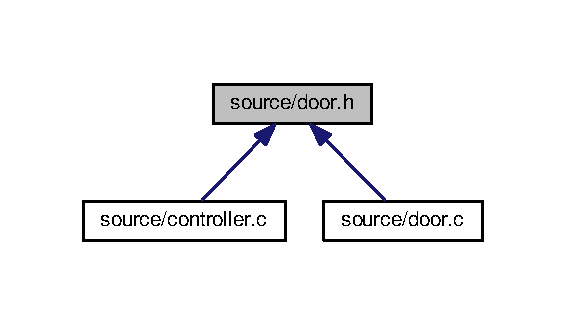
\includegraphics[width=272pt]{door_8h__dep__incl}
\end{center}
\end{figure}
\subsection*{Functions}
\begin{DoxyCompactItemize}
\item 
void \hyperlink{door_8h_a8d36b61e6e0d2ae5e0ed3ca7a7685f8f}{open\+\_\+close\+\_\+door} (\hyperlink{controller_8h_a7f15c77206bc6cf59d763bb72cc381e6}{status} $\ast$elevator)
\begin{DoxyCompactList}\small\item\em Opens the door and sets the door lamp. The door stays open for three seconds and then closes and resets door lamp. Stop button can be pressed and orders can be added to queue even though obstruction is detected. \end{DoxyCompactList}\item 
void \hyperlink{door_8h_a2eb87e0eff1a07b2039c8e17c2b272da}{check\+\_\+time} (\hyperlink{controller_8h_a7f15c77206bc6cf59d763bb72cc381e6}{status} $\ast$elevator)
\begin{DoxyCompactList}\small\item\em The timer function checks if the current time is three seconds or more from the initial time. The current time is rested if an obstruction is detected. Stop button can be pressed and orders can be added to queue even when timer is running. \end{DoxyCompactList}\end{DoxyCompactItemize}


\subsection{Detailed Description}
The door file includes functions for opening and closing the door. There is also implemented a three second time delay for holding the door open. 



\subsection{Function Documentation}
\index{door.\+h@{door.\+h}!check\+\_\+time@{check\+\_\+time}}
\index{check\+\_\+time@{check\+\_\+time}!door.\+h@{door.\+h}}
\subsubsection[{\texorpdfstring{check\+\_\+time(status $\ast$elevator)}{check_time(status *elevator)}}]{\setlength{\rightskip}{0pt plus 5cm}void check\+\_\+time (
\begin{DoxyParamCaption}
\item[{{\bf status} $\ast$}]{elevator}
\end{DoxyParamCaption}
)}\hypertarget{door_8h_a2eb87e0eff1a07b2039c8e17c2b272da}{}\label{door_8h_a2eb87e0eff1a07b2039c8e17c2b272da}


The timer function checks if the current time is three seconds or more from the initial time. The current time is rested if an obstruction is detected. Stop button can be pressed and orders can be added to queue even when timer is running. 


\begin{DoxyParams}[1]{Parameters}
\mbox{\tt in,out}  & {\em status$\ast$} & elevator Struct for elevator status. \\
\hline
\end{DoxyParams}


Definition at line 26 of file door.\+c.

\index{door.\+h@{door.\+h}!open\+\_\+close\+\_\+door@{open\+\_\+close\+\_\+door}}
\index{open\+\_\+close\+\_\+door@{open\+\_\+close\+\_\+door}!door.\+h@{door.\+h}}
\subsubsection[{\texorpdfstring{open\+\_\+close\+\_\+door(status $\ast$elevator)}{open_close_door(status *elevator)}}]{\setlength{\rightskip}{0pt plus 5cm}void open\+\_\+close\+\_\+door (
\begin{DoxyParamCaption}
\item[{{\bf status} $\ast$}]{elevator}
\end{DoxyParamCaption}
)}\hypertarget{door_8h_a8d36b61e6e0d2ae5e0ed3ca7a7685f8f}{}\label{door_8h_a8d36b61e6e0d2ae5e0ed3ca7a7685f8f}


Opens the door and sets the door lamp. The door stays open for three seconds and then closes and resets door lamp. Stop button can be pressed and orders can be added to queue even though obstruction is detected. 


\begin{DoxyParams}[1]{Parameters}
\mbox{\tt in,out}  & {\em status$\ast$} & elevator Struct for elevator status. \\
\hline
\end{DoxyParams}


Definition at line 10 of file door.\+c.


\hypertarget{queue_8h}{}\section{source/queue.h File Reference}
\label{queue_8h}\index{source/queue.\+h@{source/queue.\+h}}


The queue file includes funtions used to manipulate the queue for the elevator, determine direction based on elements in queue and check if the queue is empty.  


{\ttfamily \#include \char`\"{}elev.\+h\char`\"{}}\\*
{\ttfamily \#include \char`\"{}controller.\+h\char`\"{}}\\*
{\ttfamily \#include $<$stdbool.\+h$>$}\\*
Include dependency graph for queue.\+h\+:
\nopagebreak
\begin{figure}[H]
\begin{center}
\leavevmode
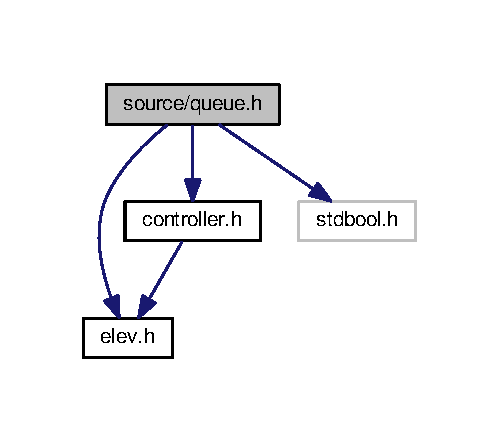
\includegraphics[width=240pt]{queue_8h__incl}
\end{center}
\end{figure}
This graph shows which files directly or indirectly include this file\+:
\nopagebreak
\begin{figure}[H]
\begin{center}
\leavevmode
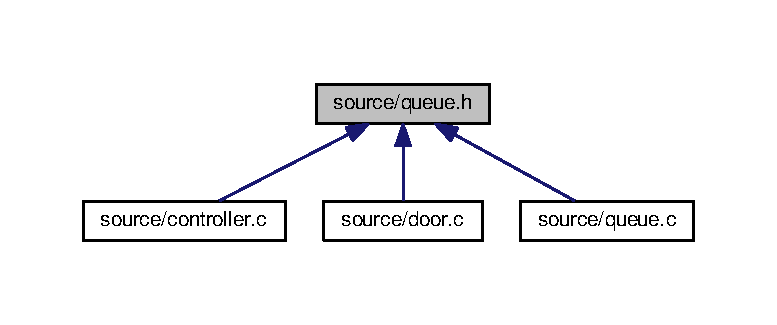
\includegraphics[width=350pt]{queue_8h__dep__incl}
\end{center}
\end{figure}
\subsection*{Functions}
\begin{DoxyCompactItemize}
\item 
int \hyperlink{queue_8h_a9137900ac5eaa00243a24012453b0bee}{stop\+\_\+dir} (\hyperlink{controller_8h_a7f15c77206bc6cf59d763bb72cc381e6}{status} $\ast$elevator)
\begin{DoxyCompactList}\small\item\em Determines the next direction for the elevator, given that the previous state was stop. The variables elevator-\/prev\+\_\+dir and elevator-\/$>$prev\+\_\+floor from status$\ast$ elevator are used to determine the direction based on the orders in the queue. \end{DoxyCompactList}\item 
elev\+\_\+motor\+\_\+direction\+\_\+t \hyperlink{queue_8h_ae26d0f526fa97ba6f4c8c5528546473c}{determine\+\_\+dir} (\hyperlink{controller_8h_a7f15c77206bc6cf59d763bb72cc381e6}{status} $\ast$elevator)
\begin{DoxyCompactList}\small\item\em Determines the next direction for the elevator. The previuos state is not taken into considerantion. The variable elevator-\/$>$current\+\_\+floor and elevator-\/$>$prev\+\_\+dir are used together with the \hyperlink{queue_8h_a9137900ac5eaa00243a24012453b0bee}{stop\+\_\+dir(status$\ast$ elevator)} funtion to determine the direction. \end{DoxyCompactList}\item 
void \hyperlink{queue_8h_a6b1bedd397488ed69e48f0d1ff97f2e5}{add\+\_\+to\+\_\+queue} (\hyperlink{controller_8h_a7f15c77206bc6cf59d763bb72cc381e6}{status} $\ast$elevator)
\begin{DoxyCompactList}\small\item\em Adds orders to the 4x3 matrix called queue in status$\ast$ elevator. The orders are added by setting the value \char`\"{}1\char`\"{} in the array if an order button is pressed. \end{DoxyCompactList}\item 
bool \hyperlink{queue_8h_a7dfc8efa12864307e80eb7b7242c01f2}{is\+\_\+queue\+\_\+empty} (\hyperlink{controller_8h_a7f15c77206bc6cf59d763bb72cc381e6}{status} $\ast$elevator)
\begin{DoxyCompactList}\small\item\em Goes through the 4x3 matrix and checks if every value is 0. \end{DoxyCompactList}\item 
void \hyperlink{queue_8h_a9ae5e8f19e9dc589a7f0eac932cd146c}{remove\+\_\+current\+\_\+floor\+\_\+from\+\_\+queue} (\hyperlink{controller_8h_a7f15c77206bc6cf59d763bb72cc381e6}{status} $\ast$elevator)
\begin{DoxyCompactList}\small\item\em Goes through the 4x3 matrix and removes every order on the current floor. \end{DoxyCompactList}\end{DoxyCompactItemize}


\subsection{Detailed Description}
The queue file includes funtions used to manipulate the queue for the elevator, determine direction based on elements in queue and check if the queue is empty. 



\subsection{Function Documentation}
\index{queue.\+h@{queue.\+h}!add\+\_\+to\+\_\+queue@{add\+\_\+to\+\_\+queue}}
\index{add\+\_\+to\+\_\+queue@{add\+\_\+to\+\_\+queue}!queue.\+h@{queue.\+h}}
\subsubsection[{\texorpdfstring{add\+\_\+to\+\_\+queue(status $\ast$elevator)}{add_to_queue(status *elevator)}}]{\setlength{\rightskip}{0pt plus 5cm}void add\+\_\+to\+\_\+queue (
\begin{DoxyParamCaption}
\item[{{\bf status} $\ast$}]{elevator}
\end{DoxyParamCaption}
)}\hypertarget{queue_8h_a6b1bedd397488ed69e48f0d1ff97f2e5}{}\label{queue_8h_a6b1bedd397488ed69e48f0d1ff97f2e5}


Adds orders to the 4x3 matrix called queue in status$\ast$ elevator. The orders are added by setting the value \char`\"{}1\char`\"{} in the array if an order button is pressed. 


\begin{DoxyParams}[1]{Parameters}
\mbox{\tt in,out}  & {\em status$\ast$} & elevator Struct for elevator status. \\
\hline
\end{DoxyParams}


Definition at line 80 of file queue.\+c.

\index{queue.\+h@{queue.\+h}!determine\+\_\+dir@{determine\+\_\+dir}}
\index{determine\+\_\+dir@{determine\+\_\+dir}!queue.\+h@{queue.\+h}}
\subsubsection[{\texorpdfstring{determine\+\_\+dir(status $\ast$elevator)}{determine_dir(status *elevator)}}]{\setlength{\rightskip}{0pt plus 5cm}elev\+\_\+motor\+\_\+direction\+\_\+t determine\+\_\+dir (
\begin{DoxyParamCaption}
\item[{{\bf status} $\ast$}]{elevator}
\end{DoxyParamCaption}
)}\hypertarget{queue_8h_ae26d0f526fa97ba6f4c8c5528546473c}{}\label{queue_8h_ae26d0f526fa97ba6f4c8c5528546473c}


Determines the next direction for the elevator. The previuos state is not taken into considerantion. The variable elevator-\/$>$current\+\_\+floor and elevator-\/$>$prev\+\_\+dir are used together with the \hyperlink{queue_8h_a9137900ac5eaa00243a24012453b0bee}{stop\+\_\+dir(status$\ast$ elevator)} funtion to determine the direction. 


\begin{DoxyParams}[1]{Parameters}
\mbox{\tt in}  & {\em status$\ast$} & elevator Struct for elevator status. \\
\hline
\end{DoxyParams}


Definition at line 35 of file queue.\+c.

\index{queue.\+h@{queue.\+h}!is\+\_\+queue\+\_\+empty@{is\+\_\+queue\+\_\+empty}}
\index{is\+\_\+queue\+\_\+empty@{is\+\_\+queue\+\_\+empty}!queue.\+h@{queue.\+h}}
\subsubsection[{\texorpdfstring{is\+\_\+queue\+\_\+empty(status $\ast$elevator)}{is_queue_empty(status *elevator)}}]{\setlength{\rightskip}{0pt plus 5cm}bool is\+\_\+queue\+\_\+empty (
\begin{DoxyParamCaption}
\item[{{\bf status} $\ast$}]{elevator}
\end{DoxyParamCaption}
)}\hypertarget{queue_8h_a7dfc8efa12864307e80eb7b7242c01f2}{}\label{queue_8h_a7dfc8efa12864307e80eb7b7242c01f2}


Goes through the 4x3 matrix and checks if every value is 0. 


\begin{DoxyParams}[1]{Parameters}
\mbox{\tt in}  & {\em status$\ast$} & elevator Struct for elevator status. \\
\hline
\end{DoxyParams}
\begin{DoxyReturn}{Returns}
T\+R\+UE if the array is empty, F\+A\+L\+SE if not empty 
\end{DoxyReturn}


Definition at line 94 of file queue.\+c.

\index{queue.\+h@{queue.\+h}!remove\+\_\+current\+\_\+floor\+\_\+from\+\_\+queue@{remove\+\_\+current\+\_\+floor\+\_\+from\+\_\+queue}}
\index{remove\+\_\+current\+\_\+floor\+\_\+from\+\_\+queue@{remove\+\_\+current\+\_\+floor\+\_\+from\+\_\+queue}!queue.\+h@{queue.\+h}}
\subsubsection[{\texorpdfstring{remove\+\_\+current\+\_\+floor\+\_\+from\+\_\+queue(status $\ast$elevator)}{remove_current_floor_from_queue(status *elevator)}}]{\setlength{\rightskip}{0pt plus 5cm}void remove\+\_\+current\+\_\+floor\+\_\+from\+\_\+queue (
\begin{DoxyParamCaption}
\item[{{\bf status} $\ast$}]{elevator}
\end{DoxyParamCaption}
)}\hypertarget{queue_8h_a9ae5e8f19e9dc589a7f0eac932cd146c}{}\label{queue_8h_a9ae5e8f19e9dc589a7f0eac932cd146c}


Goes through the 4x3 matrix and removes every order on the current floor. 


\begin{DoxyParams}[1]{Parameters}
\mbox{\tt in,out}  & {\em status$\ast$} & elevator Struct for elevator status. \\
\hline
\end{DoxyParams}


Definition at line 108 of file queue.\+c.

\index{queue.\+h@{queue.\+h}!stop\+\_\+dir@{stop\+\_\+dir}}
\index{stop\+\_\+dir@{stop\+\_\+dir}!queue.\+h@{queue.\+h}}
\subsubsection[{\texorpdfstring{stop\+\_\+dir(status $\ast$elevator)}{stop_dir(status *elevator)}}]{\setlength{\rightskip}{0pt plus 5cm}int stop\+\_\+dir (
\begin{DoxyParamCaption}
\item[{{\bf status} $\ast$}]{elevator}
\end{DoxyParamCaption}
)}\hypertarget{queue_8h_a9137900ac5eaa00243a24012453b0bee}{}\label{queue_8h_a9137900ac5eaa00243a24012453b0bee}


Determines the next direction for the elevator, given that the previous state was stop. The variables elevator-\/prev\+\_\+dir and elevator-\/$>$prev\+\_\+floor from status$\ast$ elevator are used to determine the direction based on the orders in the queue. 


\begin{DoxyParams}[1]{Parameters}
\mbox{\tt in}  & {\em status$\ast$} & elevator Struct for elevator status. \\
\hline
\end{DoxyParams}


Definition at line 7 of file queue.\+c.


%--- End generated contents ---

% Index
\backmatter
\newpage
\phantomsection
\clearemptydoublepage
\addcontentsline{toc}{chapter}{Index}
\printindex

\end{document}
